\documentclass[11pt,a4paper]{article}

\usepackage[T1]{fontenc}
\usepackage{lmodern}
\usepackage[margin=1.8cm]{geometry}
\usepackage{booktabs}
\usepackage{longtable}
\usepackage{tabularx}
\usepackage{array}
\usepackage{pdflscape}
\usepackage{subcaption}
\usepackage[table]{xcolor}
\usepackage{tikz}
\usepackage{pgfplots}
\usepackage{tcolorbox}
\usepackage{hyperref}
\usepackage{enumitem}
\pgfplotsset{compat=1.18}

\definecolor{bridge}{HTML}{2F6B9A}
\definecolor{forward}{HTML}{2E8B57}
\definecolor{direct}{HTML}{C96C2C}
\definecolor{accent}{HTML}{44546A}
\definecolor{panel}{HTML}{F4F7FA}
\definecolor{gridline}{HTML}{D8DEE8}
\definecolor{increasecolor}{HTML}{A64B2A}
\definecolor{decreasecolor}{HTML}{1F7A66}

\newcommand{\increase}[1]{\textcolor{increasecolor}{#1}}
\newcommand{\decrease}[1]{\textcolor{decreasecolor}{#1}}
\newcommand{\statbox}[2]{%
  \begin{tcolorbox}[colback=panel,colframe=accent,boxrule=0.4pt,arc=1mm,left=1mm,right=1mm,top=1mm,bottom=1mm]
  \centering{\Large\bfseries #1}\\[-1mm]{\scriptsize #2}
  \end{tcolorbox}%
}

\hypersetup{
  colorlinks=true,
  linkcolor=accent,
  urlcolor=bridge,
  pdftitle={Sigrok BMS Protocol Decoder Capture Analysis},
}

\title{Sigrok BMS Protocol Decoder Capture Analysis}
\author{Generated from offline sigrok/PulseView analysis outputs}
\date{}

\begin{document}
\maketitle

\section*{Executive Summary}

\begin{tabularx}{\textwidth}{XXXX}
\statbox{30}{total captures} &
\statbox{17}{RS485/UART captures} &
\statbox{13}{CAN captures} &
\statbox{19 / 6 / 5}{Bridge / Forward / Direct} \\
\end{tabularx}

\begin{tcolorbox}[colback=panel,colframe=accent,title=Key observations]
\begin{itemize}[leftmargin=*]
\item Anenji Pylon RS485 JKBMS shows the clearest RS485 latency change: Direct cable is -4.58 ms (-47.2\%) versus Bridge for average request-to-response latency.
\item Growatt RS485 JKBMS has slower worst-case exchange timing: Direct cable is +21.48 ms (+40.1\%) versus Bridge for full-exchange P95 latency.
\item Growatt CAN SeplosBMS cycles are shorter in Direct cable mode: Direct cable is -164.25 ms (-19.3\%) versus Bridge for average CAN cycle duration.
\item Growatt CAN JKBMS frame rate stays effectively flat across modes: Direct cable is +0.1 frames/s (+0.2\%) versus Bridge.
\end{itemize}
\end{tcolorbox}


\begin{table}[htbp]
\centering
\caption{Direct cable versus Bridge changes with at least 40\% absolute difference.}
\begingroup
\setlength{\tabcolsep}{3pt}
\begin{tabular}{@{}>{\raggedright\arraybackslash}p{5.0cm}>{\raggedright\arraybackslash}p{4.2cm}>{\raggedright\arraybackslash}p{3.2cm}@{\hspace{0.15cm}}>{\raggedright\arraybackslash}p{2.2cm}@{}}
\toprule
Group & Metric & Direct vs Bridge & Abs. change \\
\midrule
Growatt CAN JKBMS & Cycles/s & \increase{+0.1 (+100\%)} & 100\% \\
Growatt CAN JKBMS & Cycle min (ms) & \decrease{-5000.47 (-50.1\%)} & 50.1\% \\
Growatt CAN JKBMS & Cycle avg (ms) & \decrease{-5000.47 (-50.1\%)} & 50.1\% \\
Growatt CAN JKBMS & Cycle max (ms) & \decrease{-5000.47 (-50.1\%)} & 50.1\% \\
Growatt CAN JKBMS & Cycle P95 (ms) & \decrease{-5000.47 (-50.1\%)} & 50.1\% \\
Growatt CAN SeplosBMS & Cycle min (ms) & \decrease{-121.3 (-48.3\%)} & 48.3\% \\
Anenji Pylon RS485 JKBMS & Req->Rsp avg (ms) & \decrease{-4.58 (-47.2\%)} & 47.2\% \\
Growatt CAN SeplosBMS & Inter-cycle gap min (ms) & \increase{+53.56 (+46.7\%)} & 46.7\% \\
Growatt CAN SeplosBMS & Cycle max (ms) & \decrease{-664.45 (-44.4\%)} & 44.4\% \\
Anenji Pylon RS485 JKBMS & Req->Rsp P95 (ms) & \decrease{-4.22 (-42.6\%)} & 42.6\% \\
Growatt RS485 JKBMS & Full exchange P95 (ms) & \increase{+21.48 (+40.1\%)} & 40.1\% \\
\bottomrule
\end{tabular}
\endgroup
\end{table}


\section{Protocol Overview Charts}

These charts include every protocol group available in the overview CSV. Missing
topology modes are intentionally left blank, so a group can have one, two, or three
bars depending on the captures currently available.

CAN cycle duration charts use a logarithmic y-axis because values span multiple
orders of magnitude, from sub-millisecond single-frame cycles to multi-second
capture-length cycles.


\begin{figure}[p]
\centering

\begin{subfigure}{\textwidth}
\centering

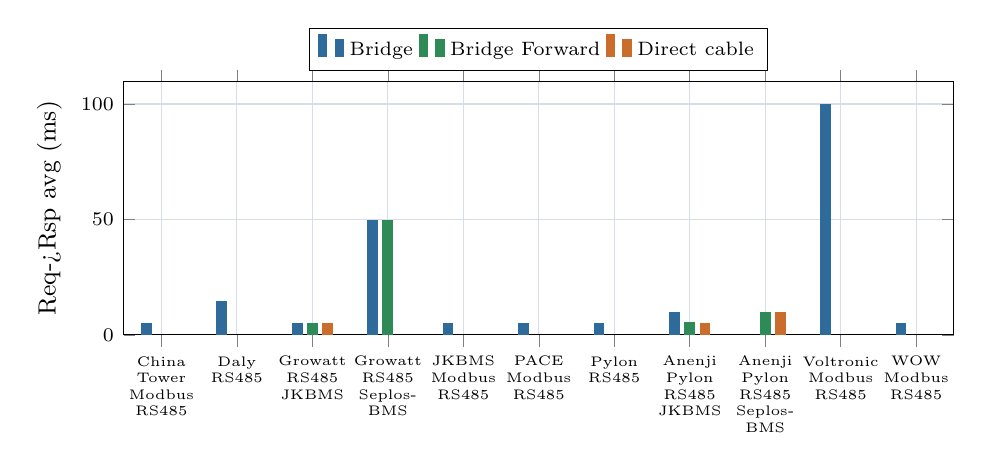
\begin{tikzpicture}
\begin{axis}[
    ybar,
    width=\textwidth,
    height=4.8cm,
    bar width=3.5pt,
    ymin=0,
    xmin=0.5,
    xmax=11.5,
    enlarge x limits=false,
    ylabel={Req->Rsp avg (ms)},
    ylabel style={font=\small},
    xtick={1,2,3,4,5,6,7,8,9,10,11},
    xticklabels={China Tower Modbus RS485,Daly RS485,Growatt RS485 JKBMS,Growatt RS485 SeplosBMS,JKBMS Modbus RS485,PACE Modbus RS485,Pylon RS485,Anenji Pylon RS485 JKBMS,Anenji Pylon RS485 SeplosBMS,Voltronic Modbus RS485,WOW Modbus RS485},
    x tick label style={text width=1.05cm, align=center, font=\tiny},
    y tick label style={font=\scriptsize},
    legend style={at={(0.5,1.04)}, anchor=south, legend columns=3, font=\scriptsize},
    grid=both,
    major grid style={draw=gridline},
]
\addplot+[fill=bridge, draw=bridge] coordinates {(1,5.015) (2,14.459) (3,4.760) (4,49.517) (5,4.904) (6,4.988) (7,4.817) (8,9.707) (10,99.797) (11,4.799)};
\addplot+[fill=forward, draw=forward] coordinates {(3,5.008) (4,49.604) (8,5.489) (9,9.470)};
\addplot+[fill=direct, draw=direct] coordinates {(3,5.127) (8,5.125) (9,9.887)};
\legend{Bridge, Bridge Forward, Direct cable}
\end{axis}
\end{tikzpicture}

\caption{Average request-to-response latency for all available RS485/UART protocol groups.}
\end{subfigure}


\begin{subfigure}{\textwidth}
\centering

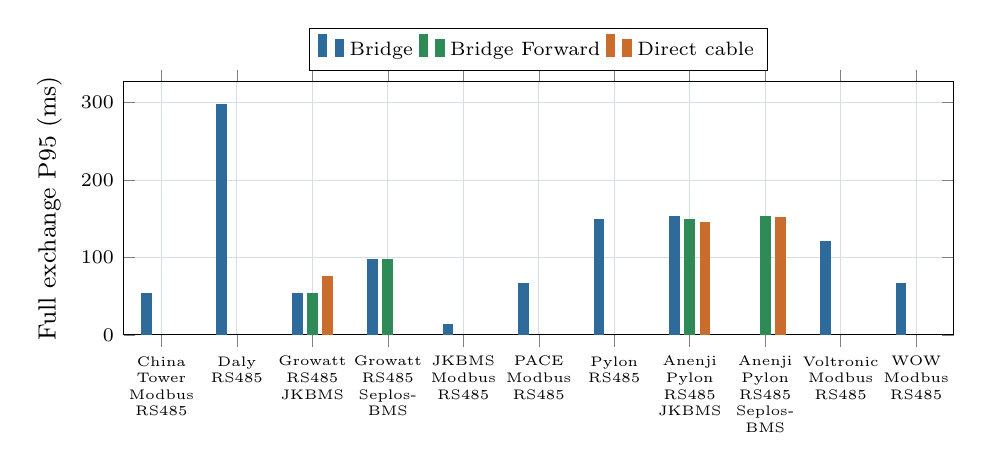
\begin{tikzpicture}
\begin{axis}[
    ybar,
    width=\textwidth,
    height=4.8cm,
    bar width=3.5pt,
    ymin=0,
    xmin=0.5,
    xmax=11.5,
    enlarge x limits=false,
    ylabel={Full exchange P95 (ms)},
    ylabel style={font=\small},
    xtick={1,2,3,4,5,6,7,8,9,10,11},
    xticklabels={China Tower Modbus RS485,Daly RS485,Growatt RS485 JKBMS,Growatt RS485 SeplosBMS,JKBMS Modbus RS485,PACE Modbus RS485,Pylon RS485,Anenji Pylon RS485 JKBMS,Anenji Pylon RS485 SeplosBMS,Voltronic Modbus RS485,WOW Modbus RS485},
    x tick label style={text width=1.05cm, align=center, font=\tiny},
    y tick label style={font=\scriptsize},
    legend style={at={(0.5,1.04)}, anchor=south, legend columns=3, font=\scriptsize},
    grid=both,
    major grid style={draw=gridline},
]
\addplot+[fill=bridge, draw=bridge] coordinates {(1,53.526) (2,297.647) (3,53.520) (4,97.806) (5,13.116) (6,66.065) (7,148.668) (8,153.034) (10,119.962) (11,65.809)};
\addplot+[fill=forward, draw=forward] coordinates {(3,53.485) (4,97.846) (8,149.320) (9,153.002)};
\addplot+[fill=direct, draw=direct] coordinates {(3,75.001) (8,145.155) (9,151.499)};
\legend{Bridge, Bridge Forward, Direct cable}
\end{axis}
\end{tikzpicture}

\caption{P95 full-exchange duration for all available RS485/UART protocol groups.}
\end{subfigure}

\caption{RS485/UART protocol overview charts.}
\end{figure}



\begin{figure}[p]
\centering

\begin{subfigure}{\textwidth}
\centering

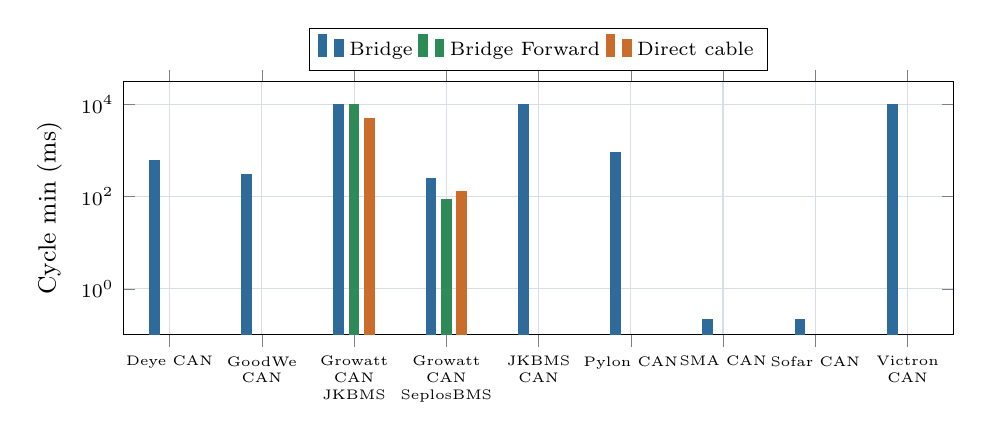
\begin{tikzpicture}
\begin{axis}[
    ybar,
    width=\textwidth,
    height=4.8cm,
    bar width=3.5pt,
    ymode=log,
    log basis y=10,
    log origin y=infty,
    ymin=0.1,
    xmin=0.5,
    xmax=9.5,
    enlarge x limits=false,
    ylabel={Cycle min (ms)},
    ylabel style={font=\small},
    xtick={1,2,3,4,5,6,7,8,9},
    xticklabels={Deye CAN,GoodWe CAN,Growatt CAN JKBMS,Growatt CAN SeplosBMS,JKBMS CAN,Pylon CAN,SMA CAN,Sofar CAN,Victron CAN},
    x tick label style={text width=1.3cm, align=center, font=\tiny},
    y tick label style={font=\scriptsize},
    legend style={at={(0.5,1.04)}, anchor=south, legend columns=3, font=\scriptsize},
    grid=both,
    major grid style={draw=gridline},
]
\addplot+[fill=bridge, draw=bridge] coordinates {(1,599.849) (2,300.246) (3,9980.699) (4,251.235) (5,9907.993) (6,900.276) (7,0.219) (8,0.219) (9,9960.726)};
\addplot+[fill=forward, draw=forward] coordinates {(3,9980.681) (4,85.691)};
\addplot+[fill=direct, draw=direct] coordinates {(3,4980.232) (4,129.933)};
\legend{Bridge, Bridge Forward, Direct cable}
\end{axis}
\end{tikzpicture}

\caption{Minimum CAN cycle duration, log scale, for all available CAN protocol groups.}
\end{subfigure}


\begin{subfigure}{\textwidth}
\centering

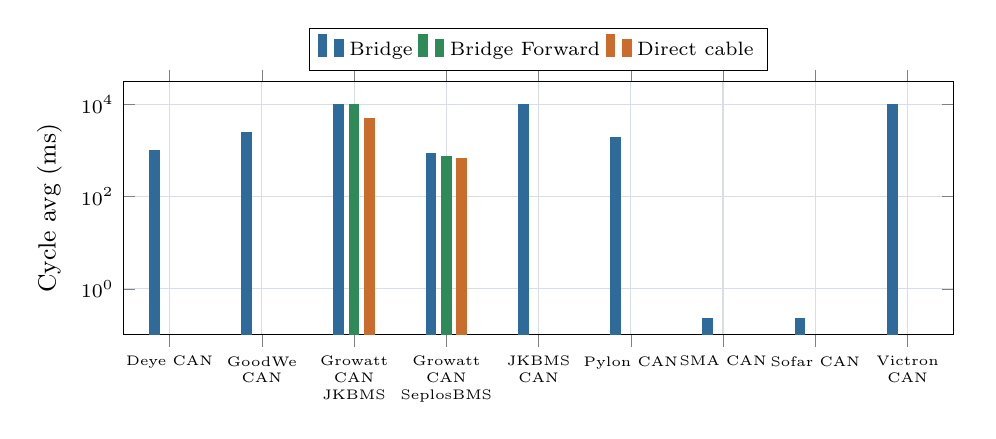
\begin{tikzpicture}
\begin{axis}[
    ybar,
    width=\textwidth,
    height=4.8cm,
    bar width=3.5pt,
    ymode=log,
    log basis y=10,
    log origin y=infty,
    ymin=0.1,
    xmin=0.5,
    xmax=9.5,
    enlarge x limits=false,
    ylabel={Cycle avg (ms)},
    ylabel style={font=\small},
    xtick={1,2,3,4,5,6,7,8,9},
    xticklabels={Deye CAN,GoodWe CAN,Growatt CAN JKBMS,Growatt CAN SeplosBMS,JKBMS CAN,Pylon CAN,SMA CAN,Sofar CAN,Victron CAN},
    x tick label style={text width=1.3cm, align=center, font=\tiny},
    y tick label style={font=\scriptsize},
    legend style={at={(0.5,1.04)}, anchor=south, legend columns=3, font=\scriptsize},
    grid=both,
    major grid style={draw=gridline},
]
\addplot+[fill=bridge, draw=bridge] coordinates {(1,1011.013) (2,2399.973) (3,9980.699) (4,851.374) (5,9907.993) (6,1900.011) (7,0.231) (8,0.229) (9,9960.726)};
\addplot+[fill=forward, draw=forward] coordinates {(3,9980.681) (4,755.942)};
\addplot+[fill=direct, draw=direct] coordinates {(3,4980.232) (4,687.126)};
\legend{Bridge, Bridge Forward, Direct cable}
\end{axis}
\end{tikzpicture}

\caption{Average CAN cycle duration, log scale, for all available CAN protocol groups.}
\end{subfigure}

\caption{CAN cycle duration overview charts.}
\end{figure}



\begin{figure}[p]
\centering

\begin{subfigure}{\textwidth}
\centering

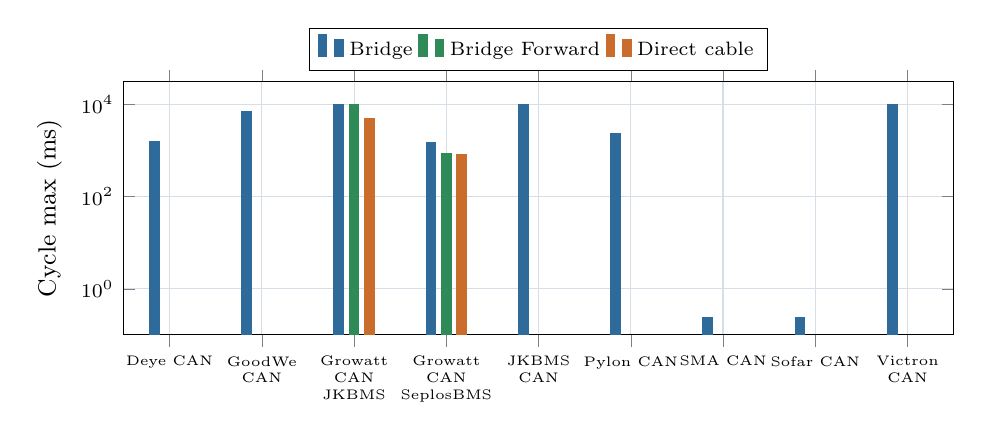
\begin{tikzpicture}
\begin{axis}[
    ybar,
    width=\textwidth,
    height=4.8cm,
    bar width=3.5pt,
    ymode=log,
    log basis y=10,
    log origin y=infty,
    ymin=0.1,
    xmin=0.5,
    xmax=9.5,
    enlarge x limits=false,
    ylabel={Cycle max (ms)},
    ylabel style={font=\small},
    xtick={1,2,3,4,5,6,7,8,9},
    xticklabels={Deye CAN,GoodWe CAN,Growatt CAN JKBMS,Growatt CAN SeplosBMS,JKBMS CAN,Pylon CAN,SMA CAN,Sofar CAN,Victron CAN},
    x tick label style={text width=1.3cm, align=center, font=\tiny},
    y tick label style={font=\scriptsize},
    legend style={at={(0.5,1.04)}, anchor=south, legend columns=3, font=\scriptsize},
    grid=both,
    major grid style={draw=gridline},
]
\addplot+[fill=bridge, draw=bridge] coordinates {(1,1599.872) (2,7100.062) (3,9980.699) (4,1496.224) (5,9907.993) (6,2299.947) (7,0.237) (8,0.237) (9,9960.726)};
\addplot+[fill=forward, draw=forward] coordinates {(3,9980.681) (4,871.815)};
\addplot+[fill=direct, draw=direct] coordinates {(3,4980.232) (4,831.769)};
\legend{Bridge, Bridge Forward, Direct cable}
\end{axis}
\end{tikzpicture}

\caption{Maximum CAN cycle duration, log scale, for all available CAN protocol groups.}
\end{subfigure}


\begin{subfigure}{\textwidth}
\centering

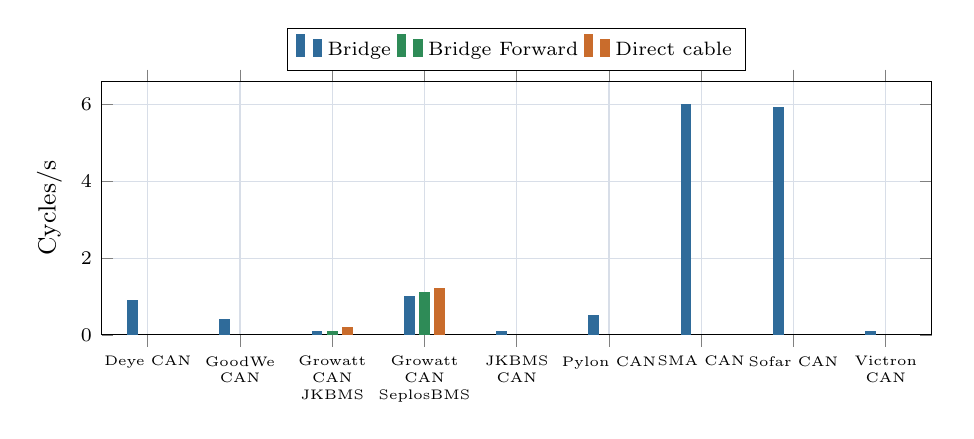
\begin{tikzpicture}
\begin{axis}[
    ybar,
    width=\textwidth,
    height=4.8cm,
    bar width=3.5pt,
    ymin=0,
    xmin=0.5,
    xmax=9.5,
    enlarge x limits=false,
    ylabel={Cycles/s},
    ylabel style={font=\small},
    xtick={1,2,3,4,5,6,7,8,9},
    xticklabels={Deye CAN,GoodWe CAN,Growatt CAN JKBMS,Growatt CAN SeplosBMS,JKBMS CAN,Pylon CAN,SMA CAN,Sofar CAN,Victron CAN},
    x tick label style={text width=1.3cm, align=center, font=\tiny},
    y tick label style={font=\scriptsize},
    legend style={at={(0.5,1.04)}, anchor=south, legend columns=3, font=\scriptsize},
    grid=both,
    major grid style={draw=gridline},
]
\addplot+[fill=bridge, draw=bridge] coordinates {(1,0.900) (2,0.400) (3,0.100) (4,1.000) (5,0.100) (6,0.500) (7,6.000) (8,5.920) (9,0.100)};
\addplot+[fill=forward, draw=forward] coordinates {(3,0.100) (4,1.100)};
\addplot+[fill=direct, draw=direct] coordinates {(3,0.200) (4,1.200)};
\legend{Bridge, Bridge Forward, Direct cable}
\end{axis}
\end{tikzpicture}

\caption{CAN cycle rate normalized by capture duration for all available CAN protocol groups.}
\end{subfigure}

\caption{CAN maximum cycle duration and throughput charts.}
\end{figure}



\begin{figure}[p]
\centering

\begin{subfigure}{\textwidth}
\centering

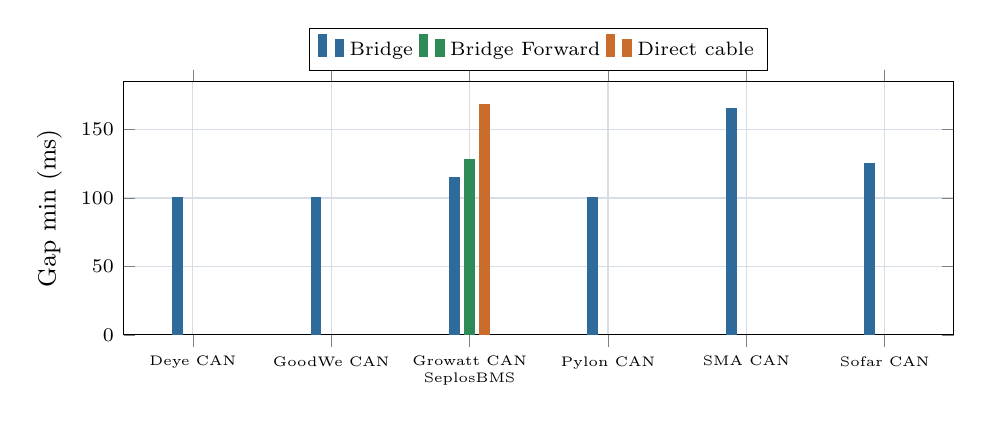
\begin{tikzpicture}
\begin{axis}[
    ybar,
    width=\textwidth,
    height=4.8cm,
    bar width=3.5pt,
    ymin=0,
    xmin=0.5,
    xmax=6.5,
    enlarge x limits=false,
    ylabel={Gap min (ms)},
    ylabel style={font=\small},
    xtick={1,2,3,4,5,6},
    xticklabels={Deye CAN,GoodWe CAN,Growatt CAN SeplosBMS,Pylon CAN,SMA CAN,Sofar CAN},
    x tick label style={text width=1.55cm, align=center, font=\tiny},
    y tick label style={font=\scriptsize},
    legend style={at={(0.5,1.04)}, anchor=south, legend columns=3, font=\scriptsize},
    grid=both,
    major grid style={draw=gridline},
]
\addplot+[fill=bridge, draw=bridge] coordinates {(1,100.186) (2,100.259) (3,114.669) (4,100.164) (5,165.308) (6,124.888)};
\addplot+[fill=forward, draw=forward] coordinates {(3,128.175)};
\addplot+[fill=direct, draw=direct] coordinates {(3,168.226)};
\legend{Bridge, Bridge Forward, Direct cable}
\end{axis}
\end{tikzpicture}

\caption{Minimum inter-cycle gap for CAN protocol groups with at least two detected cycles.}
\end{subfigure}


\begin{subfigure}{\textwidth}
\centering

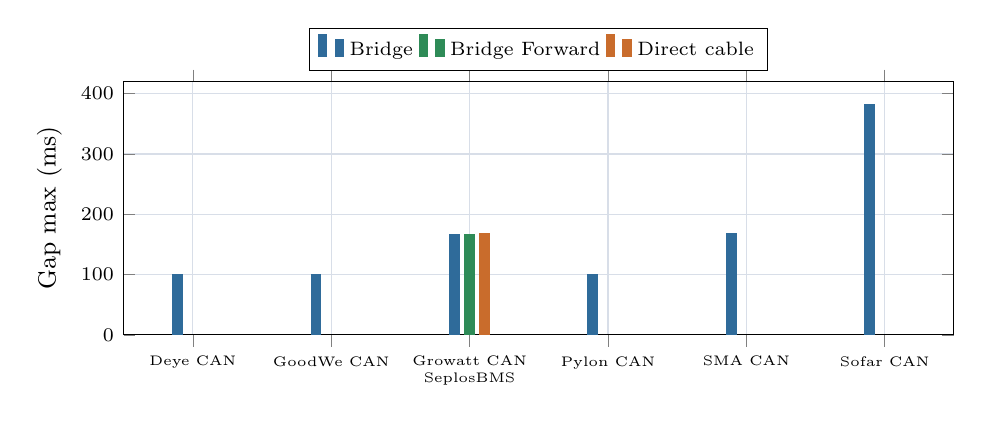
\begin{tikzpicture}
\begin{axis}[
    ybar,
    width=\textwidth,
    height=4.8cm,
    bar width=3.5pt,
    ymin=0,
    xmin=0.5,
    xmax=6.5,
    enlarge x limits=false,
    ylabel={Gap max (ms)},
    ylabel style={font=\small},
    xtick={1,2,3,4,5,6},
    xticklabels={Deye CAN,GoodWe CAN,Growatt CAN SeplosBMS,Pylon CAN,SMA CAN,Sofar CAN},
    x tick label style={text width=1.55cm, align=center, font=\tiny},
    y tick label style={font=\scriptsize},
    legend style={at={(0.5,1.04)}, anchor=south, legend columns=3, font=\scriptsize},
    grid=both,
    major grid style={draw=gridline},
]
\addplot+[fill=bridge, draw=bridge] coordinates {(1,100.204) (2,100.269) (3,165.778) (4,100.178) (5,168.242) (6,382.072)};
\addplot+[fill=forward, draw=forward] coordinates {(3,165.778)};
\addplot+[fill=direct, draw=direct] coordinates {(3,168.230)};
\legend{Bridge, Bridge Forward, Direct cable}
\end{axis}
\end{tikzpicture}

\caption{Maximum inter-cycle gap for CAN protocol groups with at least two detected cycles.}
\end{subfigure}

\caption{CAN inter-cycle gap overview charts.}
\end{figure}


\clearpage


\begin{landscape}

\section{Three-mode Delta Tables}

The following tables focus only on groups where all three modes are available: Bridge, Bridge Forward, and Direct cable. Deltas are directional: orange means an increase, green means a decrease. Timing rows are displayed in milliseconds. Whether an increase is good depends on the metric.

\subsection{RS485/UART Three-mode Deltas}
\begingroup
\scriptsize
\setlength{\tabcolsep}{3pt}
\setlength{\LTpre}{0.35em}
\setlength{\LTpost}{0.45em}
\begin{longtable}{@{}>{\raggedright\arraybackslash}p{5.0cm}>{\raggedright\arraybackslash}p{4.0cm}rrr>{\raggedright\arraybackslash}p{2.8cm}>{\raggedright\arraybackslash}p{2.8cm}>{\raggedright\arraybackslash}p{2.8cm}@{}}
\toprule
Group & Metric & Bridge & Forward & Direct & Forward vs Bridge & Direct vs Bridge & Direct vs Forward \\
\midrule
\endhead
Growatt RS485 JKBMS & Complete exchanges/s & 2.5 & 2.5 & 2 & 0 (0\%) & \decrease{-0.5 (-20\%)} & \decrease{-0.5 (-20\%)} \\
Growatt RS485 JKBMS & Req->Rsp avg (ms) & 4.76 & 5.01 & 5.13 & \increase{+0.25 (+5.2\%)} & \increase{+0.37 (+7.7\%)} & \increase{+0.12 (+2.4\%)} \\
Growatt RS485 JKBMS & Req->Rsp P95 (ms) & 5.29 & 5.29 & 5.44 & 0 (0\%) & \increase{+0.14 (+2.7\%)} & \increase{+0.14 (+2.7\%)} \\
Growatt RS485 JKBMS & Full exchange avg (ms) & 49.09 & 48.93 & 59.34 & \decrease{-0.17 (-0.3\%)} & \increase{+10.24 (+20.9\%)} & \increase{+10.41 (+21.3\%)} \\
Growatt RS485 JKBMS & Full exchange P95 (ms) & 53.52 & 53.48 & 75 & \decrease{-0.04 (-0.1\%)} & \increase{+21.48 (+40.1\%)} & \increase{+21.52 (+40.2\%)} \\
Anenji Pylon RS485 JKBMS & Complete exchanges/s & 0.8 & 0.8 & 0.8 & 0 (0\%) & 0 (0\%) & 0 (0\%) \\
Anenji Pylon RS485 JKBMS & Req->Rsp avg (ms) & 9.71 & 5.49 & 5.12 & \decrease{-4.22 (-43.5\%)} & \decrease{-4.58 (-47.2\%)} & \decrease{-0.36 (-6.6\%)} \\
Anenji Pylon RS485 JKBMS & Req->Rsp P95 (ms) & 9.91 & 6.19 & 5.69 & \decrease{-3.72 (-37.6\%)} & \decrease{-4.22 (-42.6\%)} & \decrease{-0.5 (-8\%)} \\
Anenji Pylon RS485 JKBMS & Full exchange avg (ms) & 111.16 & 106.95 & 102.92 & \decrease{-4.21 (-3.8\%)} & \decrease{-8.25 (-7.4\%)} & \decrease{-4.03 (-3.8\%)} \\
Anenji Pylon RS485 JKBMS & Full exchange P95 (ms) & 153.03 & 149.32 & 145.15 & \decrease{-3.71 (-2.4\%)} & \decrease{-7.88 (-5.1\%)} & \decrease{-4.17 (-2.8\%)} \\
\bottomrule
\end{longtable}
\endgroup





\subsection{CAN Three-mode Deltas}
\begingroup
\scriptsize
\setlength{\tabcolsep}{3pt}
\setlength{\LTpre}{0.35em}
\setlength{\LTpost}{0.45em}
\begin{longtable}{@{}>{\raggedright\arraybackslash}p{5.0cm}>{\raggedright\arraybackslash}p{4.0cm}rrr>{\raggedright\arraybackslash}p{2.8cm}>{\raggedright\arraybackslash}p{2.8cm}>{\raggedright\arraybackslash}p{2.8cm}@{}}
\toprule
Group & Metric & Bridge & Forward & Direct & Forward vs Bridge & Direct vs Bridge & Direct vs Forward \\
\midrule
\endhead
Growatt CAN JKBMS & Frames/s & 51.9 & 52 & 52 & \increase{+0.1 (+0.2\%)} & \increase{+0.1 (+0.2\%)} & 0 (0\%) \\
Growatt CAN JKBMS & Cycles/s & 0.1 & 0.1 & 0.2 & 0 (0\%) & \increase{+0.1 (+100\%)} & \increase{+0.1 (+100\%)} \\
Growatt CAN JKBMS & Cycle min (ms) & 9980.7 & 9980.68 & 4980.23 & \decrease{-0.02 (0\%)} & \decrease{-5000.47 (-50.1\%)} & \decrease{-5000.45 (-50.1\%)} \\
Growatt CAN JKBMS & Cycle avg (ms) & 9980.7 & 9980.68 & 4980.23 & \decrease{-0.02 (0\%)} & \decrease{-5000.47 (-50.1\%)} & \decrease{-5000.45 (-50.1\%)} \\
Growatt CAN JKBMS & Cycle max (ms) & 9980.7 & 9980.68 & 4980.23 & \decrease{-0.02 (0\%)} & \decrease{-5000.47 (-50.1\%)} & \decrease{-5000.45 (-50.1\%)} \\
Growatt CAN JKBMS & Cycle P95 (ms) & 9980.7 & 9980.68 & 4980.23 & \decrease{-0.02 (0\%)} & \decrease{-5000.47 (-50.1\%)} & \decrease{-5000.45 (-50.1\%)} \\
Growatt CAN SeplosBMS & Frames/s & 13 & 12.9 & 13 & \decrease{-0.1 (-0.8\%)} & 0 (0\%) & \increase{+0.1 (+0.8\%)} \\
Growatt CAN SeplosBMS & Cycles/s & 1 & 1.1 & 1.2 & \increase{+0.1 (+10\%)} & \increase{+0.2 (+20\%)} & \increase{+0.1 (+9.1\%)} \\
Growatt CAN SeplosBMS & Cycle min (ms) & 251.23 & 85.69 & 129.93 & \decrease{-165.54 (-65.9\%)} & \decrease{-121.3 (-48.3\%)} & \increase{+44.24 (+51.6\%)} \\
Growatt CAN SeplosBMS & Cycle avg (ms) & 851.37 & 755.94 & 687.13 & \decrease{-95.43 (-11.2\%)} & \decrease{-164.25 (-19.3\%)} & \decrease{-68.82 (-9.1\%)} \\
Growatt CAN SeplosBMS & Cycle max (ms) & 1496.22 & 871.81 & 831.77 & \decrease{-624.41 (-41.7\%)} & \decrease{-664.45 (-44.4\%)} & \decrease{-40.05 (-4.6\%)} \\
Growatt CAN SeplosBMS & Cycle P95 (ms) & 1221.32 & 861.95 & 831.77 & \decrease{-359.37 (-29.4\%)} & \decrease{-389.55 (-31.9\%)} & \decrease{-30.18 (-3.5\%)} \\
Growatt CAN SeplosBMS & Inter-cycle gap min (ms) & 114.67 & 128.17 & 168.23 & \increase{+13.51 (+11.8\%)} & \increase{+53.56 (+46.7\%)} & \increase{+40.05 (+31.2\%)} \\
Growatt CAN SeplosBMS & Inter-cycle gap avg (ms) & 155.49 & 160.23 & 168.23 & \increase{+4.73 (+3\%)} & \increase{+12.74 (+8.2\%)} & \increase{+8 (+5\%)} \\
Growatt CAN SeplosBMS & Inter-cycle gap max (ms) & 165.78 & 165.78 & 168.23 & 0 (0\%) & \increase{+2.45 (+1.5\%)} & \increase{+2.45 (+1.5\%)} \\
Growatt CAN SeplosBMS & Inter-cycle gap P95 (ms) & 165.78 & 165.78 & 168.23 & 0 (0\%) & \increase{+2.45 (+1.5\%)} & \increase{+2.45 (+1.5\%)} \\
\bottomrule
\end{longtable}
\endgroup

\end{landscape}


\clearpage


\begin{landscape}

\section{Capture Overview}

\subsection{RS485/UART Capture Overview}
\begingroup
\scriptsize
\setlength{\tabcolsep}{3pt}
\setlength{\LTpre}{0.35em}
\setlength{\LTpost}{0.45em}
\begin{longtable}{@{}>{\raggedright\arraybackslash}p{4.8cm}>{\raggedright\arraybackslash}p{2.35cm}rrrrrr@{}}
\toprule
Target & Topology & Frames & Complete & Incomplete & Req->Rsp avg (ms) & Req->Rsp P95 (ms) & Full P95 (ms) \\
\midrule
\endhead
China Tower Modbus RS485 & Bridge & 79 & 39 & 1 & 5.02 & 5.34 & 53.53 \\
Daly RS485 & Bridge & 88 & 44 & 0 & 14.46 & 18.06 & 297.65 \\
Growatt RS485 JKBMS & Bridge & 50 & 25 & 0 & 4.76 & 5.29 & 53.52 \\
Growatt RS485 SeplosBMS & Bridge & 49 & 24 & 1 & 49.52 & 49.86 & 97.81 \\
Growatt RS485 JKBMS & Direct cable & 100 & 50 & 0 & 5.13 & 5.44 & 75 \\
Growatt RS485 JKBMS & Bridge Forward & 50 & 25 & 0 & 5.01 & 5.29 & 53.48 \\
Growatt RS485 SeplosBMS & Bridge Forward & 49 & 24 & 1 & 49.6 & 50.49 & 97.85 \\
JKBMS Modbus RS485 & Bridge & 78 & 39 & 0 & 4.9 & 5.19 & 13.12 \\
PACE Modbus RS485 & Bridge & 79 & 39 & 1 & 4.99 & 5.26 & 66.06 \\
Pylon RS485 & Bridge & 49 & 18 & 5 & 4.82 & 5.54 & 148.67 \\
Anenji Pylon RS485 JKBMS & Bridge & 20 & 8 & 4 & 9.71 & 9.91 & 153.03 \\
Anenji Pylon RS485 JKBMS & Direct cable & 61 & 20 & 21 & 5.12 & 5.69 & 145.15 \\
Anenji Pylon RS485 SeplosBMS & Direct cable & 50 & 20 & 10 & 9.89 & 12.04 & 151.5 \\
Anenji Pylon RS485 JKBMS & Bridge Forward & 24 & 8 & 8 & 5.49 & 6.19 & 149.32 \\
Anenji Pylon RS485 SeplosBMS & Bridge Forward & 20 & 8 & 4 & 9.47 & 9.88 & 153 \\
Voltronic Modbus RS485 & Bridge & 78 & 39 & 0 & 99.8 & 101.84 & 119.96 \\
WOW Modbus RS485 & Bridge & 78 & 39 & 0 & 4.8 & 5.09 & 65.81 \\
\bottomrule
\end{longtable}
\endgroup





\subsection{CAN Capture Overview}
\begingroup
\scriptsize
\setlength{\tabcolsep}{3pt}
\setlength{\LTpre}{0.35em}
\setlength{\LTpost}{0.45em}
\begin{longtable}{@{}>{\raggedright\arraybackslash}p{4.8cm}>{\raggedright\arraybackslash}p{2.35cm}rrrrrrrr@{}}
\toprule
Target & Topology & Frames & IDs & Cycles & Cycle min (ms) & Cycle avg (ms) & Cycle max (ms) & Cycle P95 (ms) & Errors \\
\midrule
\endhead
Deye CAN & Bridge & 100 & 8 & 9 & 599.85 & 1011.01 & 1599.87 & 1599.87 & 0 \\
GoodWe CAN & Bridge & 100 & 8 & 4 & 300.25 & 2399.97 & 7100.06 & 6275.02 & 0 \\
Growatt CAN JKBMS & Bridge & 519 & 10 & 1 & 9980.7 & 9980.7 & 9980.7 & 9980.7 & 0 \\
Growatt CAN SeplosBMS & Bridge & 130 & 12 & 10 & 251.23 & 851.37 & 1496.22 & 1221.32 & 0 \\
Growatt CAN JKBMS & Direct cable & 260 & 10 & 1 & 4980.23 & 4980.23 & 4980.23 & 4980.23 & 0 \\
Growatt CAN SeplosBMS & Direct cable & 65 & 12 & 6 & 129.93 & 687.13 & 831.77 & 831.77 & 0 \\
Growatt CAN JKBMS & Bridge Forward & 520 & 10 & 1 & 9980.68 & 9980.68 & 9980.68 & 9980.68 & 0 \\
Growatt CAN SeplosBMS & Bridge Forward & 129 & 12 & 11 & 85.69 & 755.94 & 871.81 & 861.95 & 0 \\
JKBMS CAN & Bridge & 344 & 12 & 1 & 9907.99 & 9907.99 & 9907.99 & 9907.99 & 0 \\
Pylon CAN & Bridge & 100 & 8 & 5 & 900.28 & 1900.01 & 2299.95 & 2299.95 & 0 \\
SMA CAN & Bridge & 60 & 6 & 60 & 0.22 & 0.23 & 0.24 & 0.24 & 0 \\
Sofar CAN & Bridge & 148 & 6 & 148 & 0.22 & 0.23 & 0.24 & 0.24 & 0 \\
Victron CAN & Bridge & 250 & 19 & 1 & 9960.73 & 9960.73 & 9960.73 & 9960.73 & 0 \\
\bottomrule
\end{longtable}
\endgroup

\end{landscape}


\section*{Notes}

\begin{itemize}[leftmargin=*]
\item The LaTeX source is generated from committed CSV files under \texttt{analysis/out/}.
\item Capture durations are not identical, so normalized rates are included where useful.
\item CAN cycle duration can be dominated by capture length when only one cycle is detected.
\item Compiled PDFs and LaTeX build artifacts should stay out of the repository.
\end{itemize}

\end{document}
